
%% bare_conf.tex
%% V1.3
%% 2007/01/11
%% by Michael Shell
%% See:
%% http://www.michaelshell.org/
%% for current contact information.
%%
%% This is a skeleton file demonstrating the use of IEEEtran.cls
%% (requires IEEEtran.cls version 1.7 or later) with an IEEE conference paper.
%%
%% Support sites:
%% http://www.michaelshell.org/tex/ieeetran/
%% http://www.ctan.org/tex-archive/macros/latex/contrib/IEEEtran/
%% and
%% http://www.ieee.org/

%%*************************************************************************
%% Legal Notice:
%% This code is offered as-is without any warranty either expressed or
%% implied; without even the implied warranty of MERCHANTABILITY or
%% FITNESS FOR A PARTICULAR PURPOSE!
%% User assumes all risk.
%% In no event shall IEEE or any contributor to this code be liable for
%% any damages or losses, including, but not limited to, incidental,
%% consequential, or any other damages, resulting from the use or misuse
%% of any information contained here.
%%
%% All comments are the opinions of their respective authors and are not
%% necessarily endorsed by the IEEE.
%%
%% This work is distributed under the LaTeX Project Public License (LPPL)
%% ( http://www.latex-project.org/ ) version 1.3, and may be freely used,
%% distributed and modified. A copy of the LPPL, version 1.3, is included
%% in the base LaTeX documentation of all distributions of LaTeX released
%% 2003/12/01 or later.
%% Retain all contribution notices and credits.
%% ** Modified files should be clearly indicated as such, including  **
%% ** renaming them and changing author support contact information. **
%%
%% File list of work: IEEEtran.cls, IEEEtran_HOWTO.pdf, bare_adv.tex,
%%                    bare_conf.tex, bare_jrnl.tex, bare_jrnl_compsoc.tex
%%*************************************************************************

% *** Authors should verify (and, if needed, correct) their LaTeX system  ***
% *** with the testflow diagnostic prior to trusting their LaTeX platform ***
% *** with production work. IEEE's font choices can trigger bugs that do  ***
% *** not appear when using other class files.                            ***
% The testflow support page is at:
% http://www.michaelshell.org/tex/testflow/



% Note that the a4paper option is mainly intended so that authors in
% countries using A4 can easily print to A4 and see how their papers will
% look in print - the typesetting of the document will not typically be
% affected with changes in paper size (but the bottom and side margins will).
% Use the testflow package mentioned above to verify correct handling of
% both paper sizes by the user's LaTeX system.
%
% Also note that the "draftcls" or "draftclsnofoot", not "draft", option
% should be used if it is desired that the figures are to be displayed in
% draft mode.
%
\documentclass[conference]{IEEEtran}
% Add the compsoc option for Computer Society conferences.
%
% If IEEEtran.cls has not been installed into the LaTeX system files,
% manually specify the path to it like:
% \documentclass[conference]{../sty/IEEEtran}





% Some very useful LaTeX packages include:
% (uncomment the ones you want to load)


% *** MISC UTILITY PACKAGES ***
%
%\usepackage{ifpdf}
% Heiko Oberdiek's ifpdf.sty is very useful if you need conditional
% compilation based on whether the output is pdf or dvi.
% usage:
% \ifpdf
%   % pdf code
% \else
%   % dvi code
% \fi
% The latest version of ifpdf.sty can be obtained from:
% http://www.ctan.org/tex-archive/macros/latex/contrib/oberdiek/
% Also, note that IEEEtran.cls V1.7 and later provides a builtin
% \ifCLASSINFOpdf conditional that works the same way.
% When switching from latex to pdflatex and vice-versa, the compiler may
% have to be run twice to clear warning/error messages.






% *** CITATION PACKAGES ***
%
%\usepackage{cite}
% cite.sty was written by Donald Arseneau
% V1.6 and later of IEEEtran pre-defines the format of the cite.sty package
% \cite{} output to follow that of IEEE. Loading the cite package will
% result in citation numbers being automatically sorted and properly
% "compressed/ranged". e.g., [1], [9], [2], [7], [5], [6] without using
% cite.sty will become [1], [2], [5]--[7], [9] using cite.sty. cite.sty's
% \cite will automatically add leading space, if needed. Use cite.sty's
% noadjust option (cite.sty V3.8 and later) if you want to turn this off.
% cite.sty is already installed on most LaTeX systems. Be sure and use
% version 4.0 (2003-05-27) and later if using hyperref.sty. cite.sty does
% not currently provide for hyperlinked citations.
% The latest version can be obtained at:
% http://www.ctan.org/tex-archive/macros/latex/contrib/cite/
% The documentation is contained in the cite.sty file itself.


%\usepackage{algorithmic}
%\usepackage{algorithm}
%\usepackage{algpseudocode}
%\usepackage{algorithmicx}
\usepackage{listings}
\usepackage{epsfig}

\graphicspath{{figure/}}


% *** GRAPHICS RELATED PACKAGES ***
%
\ifCLASSINFOpdf
  % \usepackage[pdftex]{graphicx}
  % declare the path(s) where your graphic files are
  % \graphicspath{{../pdf/}{../jpeg/}}
  % and their extensions so you won't have to specify these with
  % every instance of \includegraphics
  % \DeclareGraphicsExtensions{.pdf,.jpeg,.png}
\else
  % or other class option (dvipsone, dvipdf, if not using dvips). graphicx
  % will default to the driver specified in the system graphics.cfg if no
  % driver is specified.
  % \usepackage[dvips]{graphicx}
  % declare the path(s) where your graphic files are
  % \graphicspath{{../eps/}}
  % and their extensions so you won't have to specify these with
  % every instance of \includegraphics
  % \DeclareGraphicsExtensions{.eps}
\fi
% graphicx was written by David Carlisle and Sebastian Rahtz. It is
% required if you want graphics, photos, etc. graphicx.sty is already
% installed on most LaTeX systems. The latest version and documentation can
% be obtained at:
% http://www.ctan.org/tex-archive/macros/latex/required/graphics/
% Another good source of documentation is "Using Imported Graphics in
% LaTeX2e" by Keith Reckdahl which can be found as epslatex.ps or
% epslatex.pdf at: http://www.ctan.org/tex-archive/info/
%
% latex, and pdflatex in dvi mode, support graphics in encapsulated
% postscript (.eps) format. pdflatex in pdf mode supports graphics
% in .pdf, .jpeg, .png and .mps (metapost) formats. Users should ensure
% that all non-photo figures use a vector format (.eps, .pdf, .mps) and
% not a bitmapped formats (.jpeg, .png). IEEE frowns on bitmapped formats
% which can result in "jaggedy"/blurry rendering of lines and letters as
% well as large increases in file sizes.
%
% You can find documentation about the pdfTeX application at:
% http://www.tug.org/applications/pdftex





% *** MATH PACKAGES ***
%
%\usepackage[cmex10]{amsmath}
% A popular package from the American Mathematical Society that provides
% many useful and powerful commands for dealing with mathematics. If using
% it, be sure to load this package with the cmex10 option to ensure that
% only type 1 fonts will utilized at all point sizes. Without this option,
% it is possible that some math symbols, particularly those within
% footnotes, will be rendered in bitmap form which will result in a
% document that can not be IEEE Xplore compliant!
%
% Also, note that the amsmath package sets \interdisplaylinepenalty to 10000
% thus preventing page breaks from occurring within multiline equations. Use:
%\interdisplaylinepenalty=2500
% after loading amsmath to restore such page breaks as IEEEtran.cls normally
% does. amsmath.sty is already installed on most LaTeX systems. The latest
% version and documentation can be obtained at:
% http://www.ctan.org/tex-archive/macros/latex/required/amslatex/math/





% *** SPECIALIZED LIST PACKAGES ***
%
%\usepackage{algorithmic}
% algorithmic.sty was written by Peter Williams and Rogerio Brito.
% This package provides an algorithmic environment fo describing algorithms.
% You can use the algorithmic environment in-text or within a figure
% environment to provide for a floating algorithm. Do NOT use the algorithm
% floating environment provided by algorithm.sty (by the same authors) or
% algorithm2e.sty (by Christophe Fiorio) as IEEE does not use dedicated
% algorithm float types and packages that provide these will not provide
% correct IEEE style captions. The latest version and documentation of
% algorithmic.sty can be obtained at:
% http://www.ctan.org/tex-archive/macros/latex/contrib/algorithms/
% There is also a support site at:
% http://algorithms.berlios.de/index.html
% Also of interest may be the (relatively newer and more customizable)
% algorithmicx.sty package by Szasz Janos:
% http://www.ctan.org/tex-archive/macros/latex/contrib/algorithmicx/




% *** ALIGNMENT PACKAGES ***
%
%\usepackage{array}
% Frank Mittelbach's and David Carlisle's array.sty patches and improves
% the standard LaTeX2e array and tabular environments to provide better
% appearance and additional user controls. As the default LaTeX2e table
% generation code is lacking to the point of almost being broken with
% respect to the quality of the end results, all users are strongly
% advised to use an enhanced (at the very least that provided by array.sty)
% set of table tools. array.sty is already installed on most systems. The
% latest version and documentation can be obtained at:
% http://www.ctan.org/tex-archive/macros/latex/required/tools/


%\usepackage{mdwmath}
%\usepackage{mdwtab}
% Also highly recommended is Mark Wooding's extremely powerful MDW tools,
% especially mdwmath.sty and mdwtab.sty which are used to format equations
% and tables, respectively. The MDWtools set is already installed on most
% LaTeX systems. The lastest version and documentation is available at:
% http://www.ctan.org/tex-archive/macros/latex/contrib/mdwtools/


% IEEEtran contains the IEEEeqnarray family of commands that can be used to
% generate multiline equations as well as matrices, tables, etc., of high
% quality.


%\usepackage{eqparbox}
% Also of notable interest is Scott Pakin's eqparbox package for creating
% (automatically sized) equal width boxes - aka "natural width parboxes".
% Available at:
% http://www.ctan.org/tex-archive/macros/latex/contrib/eqparbox/





% *** SUBFIGURE PACKAGES ***
%\usepackage[tight,footnotesize]{subfigure}
% subfigure.sty was written by Steven Douglas Cochran. This package makes it
% easy to put subfigures in your figures. e.g., "Figure 1a and 1b". For IEEE
% work, it is a good idea to load it with the tight package option to reduce
% the amount of white space around the subfigures. subfigure.sty is already
% installed on most LaTeX systems. The latest version and documentation can
% be obtained at:
% http://www.ctan.org/tex-archive/obsolete/macros/latex/contrib/subfigure/
% subfigure.sty has been superceeded by subfig.sty.



%\usepackage[caption=false]{caption}
%\usepackage[font=footnotesize]{subfig}
% subfig.sty, also written by Steven Douglas Cochran, is the modern
% replacement for subfigure.sty. However, subfig.sty requires and
% automatically loads Axel Sommerfeldt's caption.sty which will override
% IEEEtran.cls handling of captions and this will result in nonIEEE style
% figure/table captions. To prevent this problem, be sure and preload
% caption.sty with its "caption=false" package option. This is will preserve
% IEEEtran.cls handing of captions. Version 1.3 (2005/06/28) and later
% (recommended due to many improvements over 1.2) of subfig.sty supports
% the caption=false option directly:
%\usepackage[caption=false,font=footnotesize]{subfig}
%
% The latest version and documentation can be obtained at:
% http://www.ctan.org/tex-archive/macros/latex/contrib/subfig/
% The latest version and documentation of caption.sty can be obtained at:
% http://www.ctan.org/tex-archive/macros/latex/contrib/caption/




% *** FLOAT PACKAGES ***
%
%\usepackage{fixltx2e}
% fixltx2e, the successor to the earlier fix2col.sty, was written by
% Frank Mittelbach and David Carlisle. This package corrects a few problems
% in the LaTeX2e kernel, the most notable of which is that in current
% LaTeX2e releases, the ordering of single and double column floats is not
% guaranteed to be preserved. Thus, an unpatched LaTeX2e can allow a
% single column figure to be placed prior to an earlier double column
% figure. The latest version and documentation can be found at:
% http://www.ctan.org/tex-archive/macros/latex/base/



%\usepackage{stfloats}
% stfloats.sty was written by Sigitas Tolusis. This package gives LaTeX2e
% the ability to do double column floats at the bottom of the page as well
% as the top. (e.g., "\begin{figure*}[!b]" is not normally possible in
% LaTeX2e). It also provides a command:
%\fnbelowfloat
% to enable the placement of footnotes below bottom floats (the standard
% LaTeX2e kernel puts them above bottom floats). This is an invasive package
% which rewrites many portions of the LaTeX2e float routines. It may not work
% with other packages that modify the LaTeX2e float routines. The latest
% version and documentation can be obtained at:
% http://www.ctan.org/tex-archive/macros/latex/contrib/sttools/
% Documentation is contained in the stfloats.sty comments as well as in the
% presfull.pdf file. Do not use the stfloats baselinefloat ability as IEEE
% does not allow \baselineskip to stretch. Authors submitting work to the
% IEEE should note that IEEE rarely uses double column equations and
% that authors should try to avoid such use. Do not be tempted to use the
% cuted.sty or midfloat.sty packages (also by Sigitas Tolusis) as IEEE does
% not format its papers in such ways.





% *** PDF, URL AND HYPERLINK PACKAGES ***
%
\usepackage{url}
% url.sty was written by Donald Arseneau. It provides better support for
% handling and breaking URLs. url.sty is already installed on most LaTeX
% systems. The latest version can be obtained at:
% http://www.ctan.org/tex-archive/macros/latex/contrib/misc/
% Read the url.sty source comments for usage information. Basically,
% \url{my_url_here}.





% *** Do not adjust lengths that control margins, column widths, etc. ***
% *** Do not use packages that alter fonts (such as pslatex).         ***
% There should be no need to do such things with IEEEtran.cls V1.6 and later.
% (Unless specifically asked to do so by the journal or conference you plan
% to submit to, of course. )


% correct bad hyphenation here
\hyphenation{op-tical net-works semi-conduc-tor}


\begin{document}
%
% paper title
% can use linebreaks \\ within to get better formatting as desired
\title{Benchmarking FPGA High-Level Synthesis}


% author names and affiliations
% use a multiple column layout for up to three different
% affiliations
\author{\IEEEauthorblockN{
Zhihua~Li$^{\dag,\ddag}$, Colin~Yu~Lin$^\dag$, Juan~Huang$^\dag$, Yuanqiang~Li$^\dag$, Cheng~Liu$^\P$,\\
Liqun~Yang$^{\dag,\ddag}$, Hayden~Kwok-Hay~So$^\P$, and Haigang~Yang$^{\dag,\S}$}
\IEEEauthorblockA{$\dag$ System on Programmable Chip Research Department, \\Institute of Electronics, Chinese Academy of Sciences, Beijing, China\\
$\ddag$ The University of Chinese Academy of Sciences, Beijing, China\\
$\P$ Department of Electrical and Electronic Engineering, University of Hong Kong, Hong Kong\\
$\S$ Corresponding Author: yanghg@mail.ie.ac.cn}}
%Authors and Affiliations Removed for Blind Review}}

% conference papers do not typically use \thanks and this command
% is locked out in conference mode. If really needed, such as for
% the acknowledgment of grants, issue a \IEEEoverridecommandlockouts
% after \documentclass

% for over three affiliations, or if they all won't fit within the width
% of the page, use this alternative format:
%
%\author{\IEEEauthorblockN{Michael Shell\IEEEauthorrefmark{1},
%Homer Simpson\IEEEauthorrefmark{2},
%James Kirk\IEEEauthorrefmark{3},
%Montgomery Scott\IEEEauthorrefmark{3} and
%Eldon Tyrell\IEEEauthorrefmark{4}}
%\IEEEauthorblockA{\IEEEauthorrefmark{1}School of Electrical and Computer Engineering\\
%Georgia Institute of Technology,
%Atlanta, Georgia 30332--0250\\ Email: see http://www.michaelshell.org/contact.html}
%\IEEEauthorblockA{\IEEEauthorrefmark{2}Twentieth Century Fox, Springfield, USA\\
%Email: homer@thesimpsons.com}
%\IEEEauthorblockA{\IEEEauthorrefmark{3}Starfleet Academy, San Francisco, California 96678-2391\\
%Telephone: (800) 555--1212, Fax: (888) 555--1212}
%\IEEEauthorblockA{\IEEEauthorrefmark{4}Tyrell Inc., 123 Replicant Street, Los Angeles, California 90210--4321}}




% use for special paper notices
%\IEEEspecialpapernotice{(Invited Paper)}




% make the title area
\maketitle


\begin{abstract}
%\boldmath
Due to the lack of benchmarks, currently, the FPGA High Level Synthesis(HLS) tool cannot be evaluated effectively. To solve this problem, this paper develops a suit of open-source benchmarks in C/C++ format for HLS. 20 benchmarks, which cover numerous fields including network, communication, multimedia and image processing, are carefully selected from the well-known SPEC CPU 2006, MiBench, MediaBench and LINPACK benchmarks. Since the current High Level Synthesis is not supportive of specific characteristics in C/C++, to apply CPU benchmarks to HLS, modifications and refactoring of code are carried on the 20 C/C++ benchmarks without changing the original functions. During the process, this paper proposes template metaprogramming to accommodate the recursion algorithm in HLS and an efficient memory allocation algorithm to support functions for dynamically allocating memory, such as malloc. After conversion, we implement the 20 benchmarks on Vivado, Xinlinx, and evaluate the resources cost by each benchmark. The experimental results show that the benchmark suit cost BRAM from 124KB to 321451KB, DSP from 1232 to 23455,  FF from 4566 to 12256, and LUT from 2134 to 124324.
\end{abstract}
% IEEEtran.cls defaults to using nonbold math in the Abstract.
% This preserves the distinction between vectors and scalars. However,
% if the conference you are submitting to favors bold math in the abstract,
% then you can use LaTeX's standard command \boldmath at the very start
% of the abstract to achieve this. Many IEEE journals/conferences frown on
% math in the abstract anyway.

% no keywords




% For peer review papers, you can put extra information on the cover
% page as needed:
% \ifCLASSOPTIONpeerreview
% \begin{center} \bfseries EDICS Category: 3-BBND \end{center}
% \fi
%
% For peerreview papers, this IEEEtran command inserts a page break and
% creates the second title. It will be ignored for other modes.
\IEEEpeerreviewmaketitle

\section{Introduction}
%The rapid increase of complexity in system-on-chip (SoC) design requires the design community to seek design abstractions with higher productivity than register transfer level (RTL) languages. The advent of high-level synthesis (HLS) enables the automatic synthesis of high-level specifications to low-level cycle-accurate RTL specifications for efficient implementation on ASICs or FPGAs~\cite{cong2011high}. Software designers no longer need to learn unfamiliar hardware description languages and language structures. They are able to focus on algorithm and system designs with the high-level input languages such as C/C++ or SystemC. As summarized in~\cite{martin2009high}, current major commercial C-based HLS tools include Xilinx Vivado HLS~\cite{feist2012vivado} (formerly AutoPilot~\cite{zhang2008autopilot} from AutoESL), Cadence's C-to-Silicon Compiler~\cite{cadencehls}, Mentor's Catapult C~\cite{bollaert2008catapult}, Synopsys Synphony C~\cite{synopsyshls} (formerly, Synfora's PICO Express~\cite{synforatechnology}, originated from a longrange research effort in HP Labs~\cite{kucukcakar1998matisse}), Forte's Cynthesizer~\cite{meredith2008high}, and NEC's Cyber Workbench~\cite{wakabayashi2008all}. In addition, there are also free and open source tools for HLS such as C-to-Verilog~\cite{rotem2010c} and GAUT~\cite{coussy2008gaut}.

%With above various FPGA HLS tools, SoC designers have no ideas how to choose. There is no comparative measure of performance across wide range of practical benchmarks. Even a certain HLS tool is chosen and applied in the real user application, no benchmark is available to evaluate synthesis optimization techniques. In order to evaluate the performance of different commercial and academic FPGA HLS tools and synthesis optimization techniques, a synthesizable benchmark suite is required.  Since the 1990's, Multiple efforts in the area of ASIC HLS benchmarks have been made~\cite{dutt1992benchmarks,panda19951995}. More recent and open benchmark suites are CHStone~\cite{hara2008chstone} for C/C++ and S2CBench~\cite{carrions2cbench} for SystemC. However, none of them targeted for FPGA HLS tools. There is one commercial FPGA HLS benchmark suit named BDTI High-Level Synthesis Tool Certification Program~\cite{BDTIbenchmarks,benchmarkresults} which has only two benchmarks. A benchmark suite which covers various application domains is critically important for FPGA HLS tools, and it also facilitates designers to quantitatively evaluate their new ideas and algorithms.

%In this paper, we first choose 20 benchmarks in C/C++ for FPGA HLS. All benchmarks are from CPU benchmark suites, including LINPACK, MediaBench, MiBench, and SPEC CPU 2006. Selected benchmarks cover different FPGA application domains, including networking, communication, security, multimedia, image processing and so on. This benchmarks suit is available on github, http://wwww.github.com/bonelee/hls-benchmark, and it is under LGPL license.

%Currently, some important C/C++ characteristics, such as dynamic memory allocation and recursion function, are not supported by FPGA HLS tools. Besides, the pointer and array in C/C++ are only partially supported. The selected benchmarks are traditionally for CPU, and they contain these characteristics. To apply these benchmarks to FPGA HLS tools, we make some transformations to the original codes. The modifications include:
%1) separating data input and processing logic,
%2) pointer modifications,
%3) rewriting library functions, like \emph{memset}, \emph{memcpy}, \emph{strlen} and \emph{strcmp},
%4) parameterized implementations of memory dynamic allocation, such as \emph{malloc} and \emph{free},
%5) modifying some basic data structures and algorithms, for example, link list queue and hash table,
%6) changing some recursive algorithms into a non-recursive way.
%With the above modifications to the original benchmarks, this paper implements the 20 benchmarks using a state-of-the-art commercial FPGA HLS tool, Xilinx Vivado HLS, and evaluates both timing performance and resource costs of each benchmark.

%The contributions of this paper can be summarized as:
%\begin{itemize}
%  \item An open source benchmark suit in C/C++ for FPGA HLS is presented, which covers different FPGA application domains.
%  \item Code transformations are studied and implemented to
%  \item An evaluation of a state-of-the-art commercial FPGA HLS tool using the benchmark suit is presented.
%\end{itemize}

%In Section~\ref{section_related_work}, we review the evolution of ASIC and FPGA HLS benchmarks. In Section~\ref{section_benchmark_suite}, we describe features of individual programs in the presented benchmark suit. In Section~\ref{section_code_transforming}, transformation strategies applied to benchmark codes are discussed. Then, in Section~\ref{section_experiment}, we present the HLS results of our benchmarks on a Xilinx commercial tool, Vivado HLS. Finally, in Section~\ref{section_conclusions}, we conclude this paper.


The increasing design complexity pushes the design community to seek high level design abstractions with higher productivity over the conventional register transfer level (RTL). High-level synthesis (HLS), which enables the automatic synthesis of high-level specifications to low-level cycle-accurate RTL specifications for efficient implementation on ASICs and particularly FPGAs, is one of the most promising solutions. There are already a great number of HLS tools so far from both the industry and academia as summarized in~\cite{martin2009high}. 

However, the HLS tools usually could only support a subset features of an high level language and the synthesizable subset also varies a lot. Therefore, a benchmark that could fit most of the HLS tools is still greatly needed. As HLS tools target random logic synthesis, the benchmark should cover a large number of representative domains of applications. For these purposes, we build a benchmark HLS-Bench which involves 20 applications selected from LINPACK, MediaBench, MiBench, and SPEC CPU 2006. It consists of various application domains including networking, communication, security, multimedia, image processing and so on. In addition, instead of using a static data set, we have three diverse data sets for each of the application, which helps to gain insight in the scalability of the HLS tools. To make sure the benchmark be easily supported by the general HLS tools, we further performed a series of code transformation like replacing dynamic link list data structure with static arrays, changing the recursive implementation with non-recursive one, developing dynamic memory manager to support some of the \emph{malloc} and \emph{free} and so on. This benchmark suite is available \emph{HLS-Bench} under LGPL license.

Finally, we have the benchmark implemented using Xilinx Vivado HLS and evaluate the timing as well as the hardware overhead. The experiments show that the benchmark covers a distinct scale of implementations where BRAM, DSP48, FF and LUT consumption range from 124kb to 321451kb, 1232 to 23455, 4566 to 12256 and 2134 to 124324 respectively.  

The contributions of this paper can be summarized as below:
\begin{itemize}
  \item An open source benchmark suite in c/c++ for FPGA HLS is presented, which covers a wide range of application domains.
  \item Code transformations are studied and implemented to fit various HLS tools with limited syntax support.
  \item A state-of-art commercial FPGA HLS tool is evaluated using HLS-Bench.
\end{itemize}

In Section~\ref{section_related_work}, we review the evolution of both ASIC and FPGA HLS benchmarks. In Section~\ref{section_benchmark_suite}, we briefly describe features of each application in HLS-Bench. In Section~\ref{section_code_transforming}, code transformation strategies that the ease the availability of HLS tools are discussed. In Section~\ref{section_experiment}, we present the implementation results of HLS-Bench using Vivado HLS. Finally, in Section~\ref{section_conclusions}, we conclude this paper.

\section{Related Works}\label{section_related_work}

%Some of the commencing efforts were made in HLS benchmarks since the late 1980s. The HLS research community had released two standard benchmark suites for HLS in the University of California and Irvine, in 1992 and 1995, respectively. They are High Level Synthesis Workshop 1992 Benchmarks~\cite{dutt1992benchmarks} and 1995 High Level Synthesis Design Repository~\cite{panda19951995}. However, two benchmark suites are written in VHDL and not suited for FPGA HLS tools. These benchmarks had been transplanted to C in the 1990s which typically consist of less than one hundred lines of C codes. They are no longer fit for evaluating nowaday HLS tools. More complex benchmarks should be adressed in order to make HLS a really practical technology.

%Another HLS benchmark suite is the CHStone~\cite{hara2008chstone} which is presented in 2008 by Information Technology Center, Nagoya University. It consists of 12 easy-to-use programs written in C, which are selected from different application domains such as arithmetic, security, microprocessor, media processing and so on. The programs in CHStone are relatively large compared with the HLS92 and HLS95 and are very easy to use without external library. However, The main drawbacks of CHStone are as follows: 
%1)  Though there are 3 multimedia benchmarks, they are rarely involved with complex multimedia algorithms such as the encoding and decoing of image, audio and video. These algorithms are commonly used in FPGAs applications.  It is not guaranteed that the numbers of programs in CHStone are sufficient.

%2) The benchmark programs have no composite data types such as struct which is supported for most nowaday FPGA HLS tools. Furthermore, these benchmarks are not involved with dynamic memory allocation. (The author has removed the dynamic memory allocation code in benchmarks, substituting with size-fixed array.)  Neither of benchmarks involves recursion. While such features of C in HLS are desired for HLS designers. Thus, from this point of view, CHStone's benchmarks are not targeted for real HLS application scenary.  As the autor says, ``We do not intend to evaluate performance of commercial HLS tools.''

%A more recent effort for ASICs is Synthesizable SystemC Benchmark (S2CBench). It is proposed in 2013 and written in SystemC. It claims that it is to enable the direct comparison of commercial HLS tools~\cite{carrions2cbench}. It is a collection of 12+1 programs which targets a variety of applications typically used in HLS. 12 benchmarks comply with the latest SystemC synthesizable subset draft, while one design of FFT is non-synthesizable because it contains trigonometric and floating point operations. The design was added in order to help users understand how the different HLS tools support these operations as most commercial tools have different ways to support them. One of the unique features of S2CBench is that every application is accompanied by its respective testbench. However, S2CBench does not cover some application domains such as multimedia and network, none of benchmarks deals with multimedia processing algorithms.

%CHStone and S2CBench benchmarks are not targeted for FPGA HLS but ASICs HLS. However, in industry, there is a benchmark suite targeting for FPGA HLS. That is BDTI High-Level Synthesis Tool Certification Program. In 2009, Berkeley Design Technology Inc. (BDTI), an independent benchmarking and analysis firm, launched the BDTI High-Level Synthesis Tool Certification Program to evaluate high-level synthesis tools for FPGAs. It takes as their input a high-level representation of an application (written in C or MATLAB, for example) and generate a register-transfer-level (RTL) implementation for an FPGA. Two high-level synthesis tools, AutoESL's AutoPilot~\cite{zhang2008autopilot} and Synfora's PICO~\cite{synforatechnology}, have been certified under the program. BDTI's evaluation program uses two example applications, a video motion analysis application and a wireless receiver, to evaluate high-level synthesis tools. Though BDTI's two HLS benchmarks are targeted for FPGA HLS, but they just cover only video motion and wireless communication fields. It is not convinced, made someone be suspicious of the integrity and validity of evaluating FPGA HLS tools.


Some of the commencing efforts in HLS benchmarking were made in the late 1980s. High Level Synthesis Workshop 1992 Benchmarks~\cite{dutt1992benchmarks} and 1995 High Level Synthesis Design Repository~\cite{panda19951995} were two standard benchmarks released for HLS. However, HLS tools in ~\cite{dutt1992benchmarks} ~\cite{panda19951995} actually referred to compiling the HDL code to circuits and they were written in VHDL. These benchmarks were transplanted to C later, but they were tiny including less than one hundred lines of C code. Therefore, they are no longer suitable for benchmarking the latest HLS tools. 

CHStone~\cite{hara2008chstone} is then proposed to provide a more practical benchmark suite for the HLS tools. It consists of 12 easy-to-use programs written in C and includes a number of application domains such as arithmetic, security, microprocessor, media processing and so on. Moreover, the programs in CHStone are much larger compared with the HLS92 and HLS95. However, the application domain included is quite limited. Also construct data structure and dynamic memory allocation, which are removed for the HLS tools at that time, now turn to important supporting features of the latest HLS tools. In addition, just as the authors declared, CHStone doesn't intend to evaluate the commercial HLS tools. 

S2CBench written in SystemC was proposed  to enable the direct comparison of commercial HLS tools~\cite{carrions2cbench}. It consists of 12+1 programs which target a variety of applications. The 12 benchmarks comply with the latest SystemC synthesizable subset draft, while the rest one is FFT and it is non-synthesizable due to the trigonometric and floating point operations. The non-synthesizable FFT is added in order to help the users to understand how the different HLS tools work around these special occasions. Another unique feature of S2CBench is that each application is accompanied by its corresponding testbench. Nevertheless, the application domain covered in S2CBench is relatively limited. Typical applications such as Multimedia and network are not involved. 

BDTI High-Level Synthesis Tool Certification Program \textbf{citation is needed} adopts a video motion analysis application and a wireless receiver to evaluate the high-level synthesis tools. The application is big enough for evaluation but the application domain is again quite limited.  

HLS-Bench developed in this paper includes a large range of application domains. Also it have data structures and syntax supported in the latest HLS tools, which helps evaluate the HLS tools. Moreover, each application is provided with three diverse data sets and it is beneficial to gaining insight into the HLS tools.  

\section{HLS-Bench Suite}\label{section_benchmark_suite}
In this section, we present an overview of HLS-Bench, and then briefly introduce features of each application in the benchmark suite. 

\subsection{Overview}
HLS-Bench is a collection of 20 C/C++ programs selected from well-known benchmarks such as SPEC CPU2006, MiBench, MediaBench and LINPACK as shown in \ref{table_benchmark}. It covers a wide range of application domains including network, communication, safety, multimedia, image processing and so on, which are suitable for implementing on FPGA.  

On top of the broad application domains, programs involved in HLS-Bench are big enough to cover all the basic code structures like loop and condition. In addition, some of the syntax or features such as construct data structure and constant dynamic memory allocation are not well supported in earlier HLS tools, but they are gradually supported in the latest HLS tools. Therefore, they are also included in this benchmark. Finally, recursive algorithms in the benchmark that is still not supported in HLS tools are reconstructed as normal loops. \ref{table_benchmark2} presented a detailed statistic of all these features mentioned above, which will hopefully give the users an insight into the benchmark. 

\begin{table}
\caption{FPGA HLS Benchmarks}\label{table_benchmark}
\begin{tabular}{|c|c|c|}
\hline
Benchmark  & Source & Domain\tabularnewline
\hline
\hline
linpack & LINPACK Benchmark & Arithmetic\tabularnewline
\hline
astar & SPEC CPU 2006 & Network and Games\tabularnewline
\hline
qsort & MiBench & Automotive and Industrial Control\tabularnewline
\hline
stringsearch & MiBench & Office\tabularnewline
\hline
fft & MiBench & Telecomm\tabularnewline
\hline
crc32 & MiBench & Telecomm\tabularnewline
\hline
adpcm  & MiBench & Telecomm\tabularnewline
\hline
susan & MiBench & Multimedia and Consumer\tabularnewline
\hline
ispell & MiBench & Office\tabularnewline
\hline
Dijkstra & MiBench & Network\tabularnewline
\hline
bitcount & MiBench & Automotive\tabularnewline
\hline
basicmath & MiBench & Automotive and Arithmetic\tabularnewline
\hline
rijndael & MiBench & Security\tabularnewline
\hline
sha & MiBench & Security\tabularnewline
\hline
blowfish & MiBench & Security\tabularnewline
\hline
More... &  & \tabularnewline
\hline
\end{tabular}
\end{table}

\begin{table*}[!t]
\caption{FPGA HLS Benchmarks}\label{table_benchmark2}
\begin{tabular}{|c|c|c|c|c|c|c|}
\hline
Benchmark  & Lines of code & Clauses of condition & Clauses of loop & Strcut types (C struct and C++ class) & Dynamically memory allocation & Change recursion to iteration\tabularnewline
\hline
\hline
linpack & 741 & 57 & 38 & 0 & 0 & No\tabularnewline
\hline
astar & 550 & 41 & 11 & 0 & 0 & No\tabularnewline
\hline
qsort & 75 & 1 & 0 & 2 & 1 & Yes\tabularnewline
\hline
stringsearch & 407 & 25 & 27 & 0 & 0 & No\tabularnewline
\hline
fft & 385 & 10 & 7 & 0 & 0 & No\tabularnewline
\hline
crc32 & 254 & 0 & 2 & 0 & 0 & No\tabularnewline
\hline
adpcm  & 351 & 22 & 3 & 1 & 0 & No\tabularnewline
\hline
susan & 2281 & 162 & 60 & 3 & 5 & No\tabularnewline
\hline
ispell & 925 & 36 & 34 & 4 & 1 & No\tabularnewline
\hline
Dijkstra & 150 & 5 & 3 & 3 & 0 & No\tabularnewline
\hline
bitcount & 885 & 21 & 18 & 0 & 0 & Yes\tabularnewline
\hline
basicmath & 350 & 1 & 4 & 1 & 0 & No\tabularnewline
\hline
rijndael & 1767 & 36 & 33 & 1 & 0 & No\tabularnewline
\hline
sha & 350 & 6 & 14 & 1 & 0 & No\tabularnewline
\hline
blowfish & 534 & 4 & 9 & 1 & 0 & No\tabularnewline
\hline
More & TOADD &  &  &  &  & \tabularnewline
\hline
\end{tabular}

\end{table*}


\subsection{Benchmark programs}
In this section, each application included in the benchmark is briefly introduced.

(FIXME change font)linpack: It is a linear equation solver of Ax = b, where A is a dense matrix and b is a vector. It is widely used in engineering.

astar: It is a computer algorithm that is widely used in pathfinding and graph traversal. It uses a best-first search and finds a least-cost path from a given initial node to target nodes.

qsort: qsort is a classical divide and conquer algorithm and is widely used for sorting ~\cite{guthaus2001mibench}.

stringsearch: \textbf{what is the name of the stringsearch algorithm, please specify it}.

fft: It is used to perform the discrete Fourier Transform and inverse. It can convert time to frequency and vice versa and is widely used in engineering.

crc32: It is used to perform a 32-bit Cyclic Redundancy Check (CRC) on a file(FIXME). 

adpcm: Adaptive Differential Pulse Code Modulation (ADPCM) is a variation of the well-known standard Pulse Code Modulation (PCM). A typical implementation could convert 16-bit linear PCM samples to 4-bit samples, yielding a compression rate of 4:1.

susan: Susan is an image recognition package. It can be used to smooth an image and perform adjustments for threshold, brightness, and spatial control and is widely used in recognizing corners and edges in Magnetic Resonance Images of the brain. \textbf{I don't know this algorithm, but I think it is better to describe its main functionality first and typical application implemented in the benchmark later.}

ispell: Ispell is a fast spelling checker. It supports English word spell correction suggestions.

Dijkstra: Dijkstra's algorithm is a well known solution to the shortest path problem and can be completed in O($n^2$) time.

basicmath: The basic math program includes a group of typical mathematical calculations such as cubic function solving, integer square root as well as degree and radian conversion.

bitcount: The bitcount program is used to count the number of bits of an integer. Five different algorithms including an optimized 1-bit per loop counter, recursive bit count by nibbles, non-recursive bit count by nibbles using a look-up table, non-recursive bit count by bytes using a look-up table and shifting and accumulation \textbf{not sure about the last algorithms described here, please double check}.

rijndael encrypt/decrypt: Rijndael is a block cipher with the option of 128-bit, 192-bit and 256-bit keys and blocks. It is in the National Institute of Standards and Technologies Advanced Encryption Standard (AES). 

sha: SHA is a secure hash algorithm and it will produce a 160-bit message digest for a given input. It is widely used for cryptographic key exchange, digital signature generation and well-known MD4 and MD5 hashing.

blowfish encrypt/decrypt: Blowfish is a symmetric block cipher with a variable length key. Its key length ranges from 32 to 448 bits and it is suitable for domestic and exportable encryption.

patricia: a patricia trie is an efficient data structure to represent full trees with sparse leaf nodes. It helps reduce the traversal time, and are typically used to implement routing tables in network applications. 

h263enc/h263dec: H.263 is a video compression standard originally designed as a low-bitrate compressed format for video conferencing. h263enc and h263dec are used for encoding and decoding respectively.

mp3enc/mp3dec: They come from LAME benchmark in Mibench. LAME is a free software codec used to encode/compress audio into the lossy MP3 file format. 
Mp3enc encodes a raw (headerless) PCM stream or Waveform Audio File Format (commonly known as WAV due to its filename extension) to MP3. It supports constant, average and variable bit-rate encoding. Mp3dec decodes the input MP3 to WAV or raw PCM format.

\section{Code Transformations}\label{section_code_transforming}
As the benchmarks are selected from conventional CPU benchmarks, some of them can't be used for FPGA HLS directly. Therefore, refactoring and modification are crucial for implementing these algorithms using FPGA HLS tools. While these processing is actually what a software developer may confront using HLS tools, we detail the processing in this section. Hopefully, it may help the software developer to access the FPGA HLS tools.

\subsection{Code Refactoring}
As FPGA HLS tools couldn't support file reading and writing, they are removed from the original source code and replaced with \textbf{How did you replace the file reading and writing? What do you mean by data processing and controlling? On top of the file reading and writing, are there any other "data controlling"?}. Execution time extraction code which is useless for FPGA HLS is also removed accordingly.
%Code refactoring is the process of restructing existing computer code - changing the factoring - that either presevers the behavior of the software, or at least does not modify its conformance to functional requirements~\cite{fowler1999refactoring}. It improves the code readability and reduced complexity, making the source code of more maintainability and extensibility. Some of choosed CPU benchmarks code mixed data process logic with the data input (such as read processing data from file which is not synthesizable by FPGA HLS tools) or output (such as write processed data to file or add some timing function to calculate the procecure executing time). We have to take the data process logic apart and let it be the FPGA HLS benchmark. Besides, some functions of the benchmarks are too long, we trimed them with severval smaller functions. Good news is that most CPU benchmarks have test input file and the golden result output file,  we can quickly find the error of illegal code modifications. So the code refactoring work is of not too much impedient.

\subsection{Pointer}
\label{subsection-pointer}
A pointer is an address to a location in memory and it can used as function parameters, array handling, pointer to pointer, and type casting. Despite of the convenience brought by the pointer, FPGA HLS tools could mainly support the pointers that are known at compilation time. While the pointers that are known at runtime are just partially supported at the moment. Figure \ref{Unsupported-Dynamic-Memory} and Figure \ref{Supported-Pointer-in-HLS} present two typical code styles that are un-synthesizable and synthesizable respectively.

\begin{figure}[htb]\centering
{\fontsize{8}{8}\selectfont
\begin{lstlisting}[frame=lines]
int *pointer_runtime = malloc(sizeof(int) * 100);
\end{lstlisting}
}
\caption{Unsupported Dynamic Memory Allocation in HLS}\label{Unsupported-Dynamic-Memory}
\end{figure}

\begin{figure}[htb]\centering
{\fontsize{8}{8}\selectfont
\begin{lstlisting}[frame=lines]
int data[100];
int *pointer_to_data = data;
\end{lstlisting}
}
\caption{Supported Pointer in HLS: Managing Array Access with a Pointery}\label{Supported-Pointer-in-HLS}
\end{figure}

Although dynamic pointers are not well supported inner the function to be synthesized, they can actually be perfectly synthesized at the interface. The pointers at the interface can either be synthesized as a memory-mapped IO or stream IO. For memory mapped IO, it is required to specify the memory size at compilation time. Fortunately, you can specify it using the compilation pragma or directives instead of source code directly. If it is a streamed IO, hand shaking protocol will be synthesized and you don't have to specify the size of the input. Figure \ref{Unsynthesizable-code} and Figure \ref{Supported-Pointer-in-HLS} are examples of dynamic pointer synthesis at the interface.

\begin{figure}[htb]\centering
{\fontsize{8}{8}\selectfont
\begin{lstlisting}[frame=lines]
int accumulate1(int *data,int length) {
    int sum = 0;
    for (int i = 0; i < length; ++i) {
        sum += data[i];
    }
    return sum;
}
\end{lstlisting}
}
\caption{Unsynthesizable code: accumulate an array}\label{Unsynthesizable-code}
\end{figure}


\begin{figure}[htb]\centering
{\fontsize{8}{8}\selectfont
\begin{lstlisting}[frame=lines]
#define LENGTH 100
int accumulate2(int data[LENGTH]) {
    int sum = 0;
    for (int i = 0; i < LENGTH; ++i) {
        sum += data[i];
    }
    return sum;
}
\end{lstlisting}
}
\caption{Synthesizable code: accumulate an array.}\label{Synthesizable-code}
\end{figure}

As explained above, the dynamic pointers inner the function to be synthesized in the benchmark source code are replaced with static allocation. The ones at the interface will be left unchanged.

\subsection{Library Functions}
There are many C string and memory library functions such as memset, memcpy, strlen and strcmp in the original benchmark. Although they can actually be implemented on FPGA, they are not supported in FPGA HLS tools at the moment. To bridge this gap, we develop a synthesizable library for the benchmarks so that the original can be updated with minimal efforts. Figure \ref{hls_strlen} shows a simple example on how the synthesizable library be used.

\begin{figure}[htb]\centering
{\fontsize{8}{8}\selectfont
\begin{lstlisting}[frame=lines]
#define MAX_CHAR_SIZE 1024

unsigned hls_strlen(char string[MAX_CHAR_SIZE]) {
    unsigned length = 0;
    for (length = 0; string[length] != 0; ++length);
    return length;
}
\end{lstlisting}
}
\caption{Rewrited HLS strlen Function.}\label{hls_strlen}
\end{figure}

\subsection{Dynamic Memory Allocation}\label{section_malloc}
Dynamic memory allocation is one of the typical memory management techniques in C and C++ programming languages. It can be used to allocate or release resource as needed at runtime. Essentially, this feature helps to share the limited physical memory. However, when the dynamic memory behaviour is compiled from high level language program to FPGA using HLS tools, it is actually different, though the synthesized hardware may still maintain the same functionality of the original program. The main reason is that the declared memory is implemented in a static way on FPGA and can't be released until the FPGA is reconfigured.

\begin{figure}[htb]\centering
{\fontsize{8}{8}\selectfont
\begin{lstlisting}[frame=lines]
int array[100];
\end{lstlisting}
}
\caption{HLS-Compliant Automatic Memory Allocation}\label{Automatic-Memory-Allocation}
\end{figure}

\begin{figure}[htb]\centering
{\fontsize{8}{8}\selectfont
\begin{lstlisting}[frame=lines]
static int array[100];
\end{lstlisting}
}
\caption{HLS-Compliant Static Memory Allocation}\label{Static-Memory-Allocation}
\end{figure}

\begin{figure}[htb]\centering
{\fontsize{8}{8}\selectfont
\begin{lstlisting}[frame=lines]
int *array = malloc(sizeof(int) * allocated_size);
\end{lstlisting}
}
\caption{Dynamic Memory Allocation}\label{Dynamic-Memory-Allocation}
\end{figure}

To keep the memory behaviour the same with that described in high level language program, we develop a memory allocation algorithm that could support dynamic memory allocation and sharing as software. The dynamic memory allocation algorithm is detailed in Algorithm \ref{algorithm_hls_malloc}. First of all, we declare a static array which can be synthesized as a shared static memory using FPGA HLS tools. Then the shared memory is divided into multiple chunks logically and the availability of each chunk of the memory is recorded in a bitmap as shown in Figure \ref{fig_bitmap}. Whenever there is a memory allocation request, corresponding amount of memory is allocated in chunks and the bitmap is updated as well. When the allocated memory is released, the bits in bitmap are reset accordingly. \textbf{As the mmeory allocation and release are usually sequential, the memory manger is actually simple and will not cost much hardware. In addition, bitmap is small even when the chunk size is tiny, thus the overhead can be negligible.} While the main challenge is the size of the pre-allocated shared memory, because it must be big enough to meet all the memory allocations request involved. And the exact number depends on the target benchmark. 

\begin{figure}[htb]\centering
    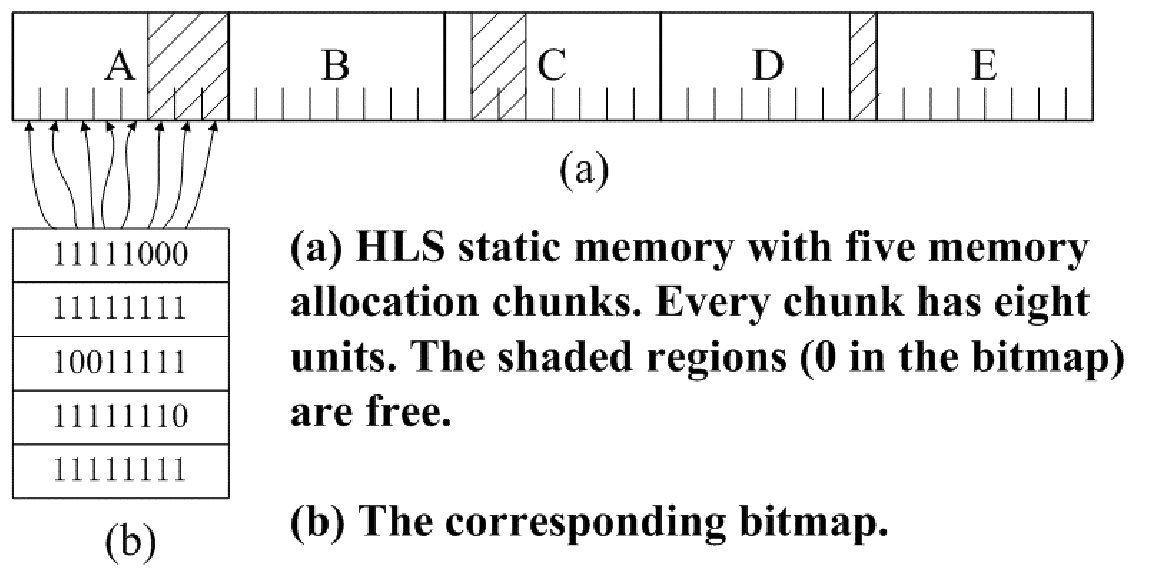
\includegraphics[scale=0.3]{bitmap}\\
    \caption{TODO FIXME (a) HLS static memory with five memory allocation chunks. Every chunk has eight units. The shaded regions (0 in the bitmap) are free. (b) The corresponding bitmap.}    \label{fig_bitmap}
\end{figure}

\begin{figure}[htb]\centering
{\fontsize{6}{6}\selectfont
\begin{lstlisting}[frame=lines]
Prerequisite:
M, pre-allocated static memory
B, bitmap for allocation chunks, all bits initialized with 0
K, user requested K units memory at runtime
S, memorizing allocated memory, used for deallocate

Seek for K consecutive 0 bits in the bitmap B.
Let the found location be F.
Set K consecutive 0 bits to 1 at the beginning F in bitmap B.
Return the corresponding location in M to the location F of bitmap B.
Record F, K and the above returned result in S.
\end{lstlisting}
}
\caption{(TODO, FIXME) Dynamic Memory Allocation Algorithm in HLS}\label{algorithm_hls_malloc}
\end{figure}


%The proposed memory allocation algorithm makes the A bitmap provides a simple way to keep track of memory in a fixed amount of memory because the size of the bitmap depends only on the size of memory and the size of the allocation chunk. The size of the allocation chunks is an important design issue. The smaller the allocation chunk, the larger the bitmap. During FPGA HLS design, the static memory is stored externally. What this can often imply when hardware is synthesized is that either the data in memory is expected every clock cycle, or there is some sort of off-chip storage in either registers or memory. More memory allocation chunks can increase data access parallelism in the HLS generated implementation. However, even with an unit as small as 4 bytes, 32 bits of memory will require only 1 bit of the map. A memory of 32n bits will use n map bits, so the bitmap will take up only 1/33 of memory. If the allocation chunk is chosen large, the bitmap will be smaller and has an adverse effect on data access parallelism in FPGA HLS design.



%\begin{figure}[h]\centering
%{\fontsize{8}{8}\selectfont
%\begin{algorithmic}
%%\textbf{Prerequisite}:
%%\STATE M, the pre-allocated static memory
%%\STATE B, the bitmap for allocation chunks, all bits initialized with 0
%%\STATE K, the user requested K units memory at runtime
%%\STATE S, memorizing allocated memory, used for deallocate
%%
%%\STATE Seek for K consecutive 0 bits in the bitmap B.
%%\STATE Let the found location be F.
%%\STATE Set K consecutive 0 bits to 1 at the beginning F in bitmap B.
%%\STATE Return the corresponding location in M to the location F of bitmap B.
%%\STATE Record F, K and the above returned result  in S.
%\end{algorithmic}
%}
%\caption{(TODO, FIXME) Dynamic Memory Allocation Algorithm in HLS}\label{algorithm_hls_malloc}
%\end{figure}

%
%int accumulate3(int (&data)[LENGTH]) {
%    int sum = 0;
%    for (int i = 0; i < LENGTH; ++i) {
%        sum += data[i];
%    }
%    return sum;
%}
%
%template<int length>
%int accumulate(int (&data)[length]) {
%    int sum = 0;
%    for (int i = 0; i < length; ++i) {
%        sum += data[i];
%    }
%    return sum;
%}
%
%int accumulate4(int (&data)[LENGTH]) {
%    return accumulate(data);
%}
%
%

\subsection{Data Structure and Algorithm Modifications}
%In some cases when applying the CPU benchmarks to FPGA HLS, we have to modify the basic data structures utilized in these benchmarks. The reason lies in that the current HLS compiler constrains the use of pointer, which makes it unable to use the pointer variable in the C/C++ struct. This means that the HLS can not use the data structure like list, which usually contains the pointer variables pointing to the next node in one of its nodes' struct. Thus, we have to modify the list and the corresponding algorithm of the benchmarks which use it. Since the HLS compiler supports fixed-size data array, the data array can be utilized to replace list. Employing this idea, we do modifications to the benchmarks as follows.
%1) We realize the queue in dijkstra CPU benchmark with array instead of the list.
%2) The original hash table data structure in ispell benchmark utilized list to solve the collision existing in hash, whereas we make use of quadratic probing to achieve this and employ the way based on array copy to realize the rehasing by using the HLS dynamically allocating algorithm discussed in section \ref{section_malloc}.
Dynamic data structures such as list constructed with link list are not supported by the HLS tools, and they are re-implemented using static data structures like array instead. Note that the array can be allocated dynamically taking advantage of the proposed dynamic memory allocation algorithm as discussed in section \ref{section_malloc}. 

%在将CPU benchmarks应用于FPGA HLS的过程中,少数情况下我们不得不修改基本benchark中表示的基本数据结构。
%根本原因在于当前HLS compiler对指针使用的限制,你无法在C/C++ struct中使用指针变量。
%这意味着HLS程序无法使用像链表这样的数据结构,因为链表的节点struct中通常包含指向下一节点的指针成员变量。
%对于那些在程序中使用了链表数据结构的benchmarks,我们不得不修改这些数据结构和对应的算法。
%好在HLS compiler支持固定大小的数组,通常情况下,可以使用数组来替代链表这样的数据结构。例如:
%1)在对dijkstra CPU benchmark里,我们将list实现的queue转换为array实现!
%2)在ispell benchmark里,其原有的hashtale数据结构是采用链表来解决hash的冲突,而我们使用平方探测法(quadratic probing)来解决hash冲突,
%并使用基于array复制的方式来实现再散列(rehashing)。//FIXME add hls-mem-manager
%修改benchmark数据结构是一个比较困难且很耗时的工作,因为我们必须在理解大部分代码(尤其是那些涉及关键数据结构和算法的代码)的基础上
%进行修改,好在原有的CPU benchmark包含了测试集和黄金测试结果(golden result),使得我们对于代码的正确修改得到了保证。


\subsection{Recursive Algorithm}
%Recursion is the process a procudure goes through when one of the steps of the procecure involves invoking the procecure itself. A procecure that goes through recursion is said to be recursive. As a computer programming technique, this is called divide and conquer and is key to the design of  many important algorithms.

Recusion provides an effective way to implement many recursive algorithms. However, its dynamic characteristic makes it tricky for hardware design let alone HLS tools. Therefore, all the recursive implementation is replaced with a plain loop instead. Figure \ref{figure_qsort_recursive} and \ref{figure_qsort_iterative} give an example how a recursive quicksort algorthm is implemented using plain loop.

\begin{figure}[htb]\centering
{\fontsize{8}{8}\selectfont
\begin{lstlisting}[frame=lines]
quicksort(array, low, high):
  if low < high:
    p := partition(array, low, high)
    quicksort(array, low, p - 1)
    quicksort(array, p + 1, high)
\end{lstlisting}
}
\caption{Pseudocode of Recursive quick sort Function.}\label{figure_qsort_recursive}
\end{figure}

\begin{figure}[htb]\centering
{\fontsize{8}{8}\selectfont
\begin{lstlisting}[frame=lines]
iterative-quicksort(array, low, high):
  create an auxiliary stack SA to store low, high
  push initial values of low and high to SA
  while SA is not empty:
    pop high and low from stack SA
    p := partition(array, low, high)
    if (p - 1) > low:
      push low and (p - 1) to stack
    if (p + 1) < high:
      push (p + 1) an high to stack
\end{lstlisting}
}
\caption{Pseudocode of iterative quck sort Function.}\label{figure_qsort_iterative}
\end{figure}

%Some specific recursion can be solved to obtain a non-recursive definition such as the iterative quick sort discussed above. In some cases, it is hard even impossible to ``translate" from recursion to non-recursion. But there is not much complex recursion in CPU benchmarks during our transforming code work.
% A classic example of recursion is the definition of the factorial function, given in Figure \ref{figure_fact} in C code.
%
%\begin{figure}[h]\centering
%{\fontsize{8}{8}\selectfont
%\begin{lstlisting}[frame=lines]
%unsigned factorial(unsigned n) {
%    if (n == 0) {
%        return 1;
%    } else {
%        return n* factorial(n-1);\
%    }
%}
%\end{lstlisting}
%}
%\caption{Recursive factorial Function.}\label{figure_fact}
%\end{figure}
%
%The function calls itself recursively on a smaller version of the input (n-1) and multiplies the result of the recursive call by n, until reaching the base case, analogously to the mathematical definition of factorial.
%
%However, recursion is not supported by nowaday hls compiler. Some specific recursion can be solved to obtain a non-recursive definition. The recursive version of factorial can be modified with iterative version.

\section{Experiments}\label{section_experiment}
In this section, we have HLS-Bench synthesized using the latest commercial HLS tools and then the hardware overhead of the benchmark is analyzed.

In the experiments, Xilinx Vivado HLS ~\cite{feist2012vivado} (2013.4 Version) is used. xc7v2000tflg1925-1, which is large enough as shown in \ref{table_available_resources} to accommodate any of the application in the benchmark, is chosen as the target device. Timing constrain is set to be 100MHz and default synthesis options are used directly. \textbf{I guess it will be better to have some basic optimization strategy such as interface setup? loop unrolling strategy? pipelined or not?. But it seems that we don't have time to do that...}

%The available resources on this chip are summarized in table . The BRAM Block (BRAM) is a configurable memory module that attaches to a variety of BRAM Interface Controllers. It is a dual-port RAM module instantiated into the FPGA fabric to provide on-chip storage for a relatively large set of data. The type of BRAM memories available in xc7v2000tflg1925-1 device can hold either 18k bits. The DSP48E block is an arithmetic logic unit (ALU) embedded into the fabric of the FPGA. It supports many independent functions of digital signal processing. These functions include multiply, multiply accumulate (MACC), multiply add and so on. As shown in table \ref{table_available_resources},  the DSP48E block in xc7v2000tflg1925-1 device available  is 2160.
%

\begin{table}[htb]
\caption{Available resources of xc7v2000tflg1925-1}\label{table_available_resources}
\begin{tabular}{|c|c|c|c|}
\hline
BRAM\_18K & DSP48E & Flip-Flop & LUT\tabularnewline
\hline
\hline
2584 & 2160 & 2443200 & 1221600\tabularnewline
\hline
\end{tabular}
\end{table}

%During experiment, We set the target clock period to 10ns, and other options to default. Beisides, we do not do optimizations on benchmarks during the experiment. The sythesis result for FPGA HLS benchmark programs are shown in Table \ref{table_systhesis_result}.

%


\begin{table*}[!t]
\caption{Sythesis result for FPGA HLS benchmark programs}\label{table_systhesis_result}

\begin{tabular}{|c|c|c|c|c|c|c|}
\hline
Benchmark & Input & Timing Estimates & \multicolumn{1}{c}{} & \multicolumn{1}{c}{Utilization} & \multicolumn{1}{c}{Estimates} & \tabularnewline
\cline{3-7}
Feature & Parameters & Clock Period (ns) & BRAM\_18K  & DSP48E  & FF & LUT\tabularnewline
\hline
\hline
linpack & N=50 & 8.7 & 0 & 114 & 11307 & 13738\tabularnewline
\cline{2-7}
Solve ax=b with matrix dimension size N of b & N=100 & 8.7 & 0 & 114 & 11522 & 14018\tabularnewline
\cline{2-7}
 & N=1000 & 8.7 & 0 & 114 & 12184 & 14824\tabularnewline
\hline
Dijkstra & N=10 & 7.98 & 451 & 0 & 402 & 975\tabularnewline
\cline{2-7}
Calculates the shortest path between every pair of nodes & N=100 & 7.98 & 482 & 1 & 478 & 1080\tabularnewline
\cline{2-7}
in a graph represented by adjacency matrix with size N$\times$N & N=1000 & 7.98 & 2436 & 1 & 551 & 1190\tabularnewline
\hline
qsort & N=1000 & 7.92 & 35 & 0 & 1861 & 2367\tabularnewline
\cline{2-7}
Sorts an array with size N & N=5000 & 7.92 & 35 & 0 & 1910 & 2404\tabularnewline
\cline{2-7}
 & N=10000 & 7.92 & 35 & 0 & 1929 & 2417\tabularnewline
\hline
stringsearch & N=1k & 7.12 & 2 & 0 & 644 & 1135\tabularnewline
\cline{2-7}
Searches for given words with total length N & N=4k & 7.12 & 3 & 0 & 652 & 1147\tabularnewline
\cline{2-7}
 & N=16k & 7.12 & 9 & 0 & 660 & 1159\tabularnewline
\hline
fft & N=1M & 8.64 & 19 & 73 & 10057 & 17936\tabularnewline
\cline{2-7}
Performs a Fast Fourier Transform & N=4M & 8.64 & 19 & 73 & 10103 & 17983\tabularnewline
\cline{2-7}
 on an array of data with size N & N=16M & 8.64 & 19 & 73 & 10149 & 18028\tabularnewline
\hline
crc32 & N=1M & 5.62 & 1 & 0 & 104 & 191\tabularnewline
\cline{2-7}
Performs a 32-bit Cyclic Redundancy Check & N=4M & 5.62 & 1 & 0 & 108 & 197\tabularnewline
\cline{2-7}
 on an array of data with size N & N=16M & 5.62 & 1 & 0 & 112 & 204\tabularnewline
\hline
adpcm & N=1M & 8.47 & 4 & 0 & 809 & 2056\tabularnewline
\cline{2-7}
Takes 16-bit linear PCM samples and converts them to 4-bit & N=4M & 8.47 & 4 & 0 & 811 & 2062\tabularnewline
\cline{2-7}
samples. The input samples are an array of data with size N & N=16M & 8.47 & 4 & 0 & 813 & 2068\tabularnewline
\hline
astar & N=20 & 8.53 & 15 & 28 & 3549 & 9432\tabularnewline
\cline{2-7}
Finds a least-cost path from a given initial node to & N=60 & 8.53 & 78 & 28 & 3620 & 9513\tabularnewline
\cline{2-7}
 one goal node in the map with width and height N & N=100 & 8.53 & 295 & 30 & 3754 & 9516\tabularnewline
\hline
susan & N=1k & 8.44 & 300 & 98 & 14764 & 28029\tabularnewline
\cline{2-7}
Smooth an image and has adjustments for threshold, brightness,  & N=4k & 8.44 & 300 & 98 & 14934 & 28427\tabularnewline
\cline{2-7}
and spatial control. The image data is in an array with size N. & N=16k & 8.44 & 300 & 98 & 15104 & 28825\tabularnewline
\hline
ispell & N=100 & 7.92 & 110 & 10 & 4598 & 8038\tabularnewline
\cline{2-7}
Spelling checker for English words in a word array with size N. & N=1000 & 7.92 & 110 & 10 & 4610 & 8054\tabularnewline
\cline{2-7}
 & N=10000 & 7.92 & 110 & 10 & 4635 & 8108\tabularnewline
\hline
rijndael & N=1k & 8.34 & 40 & 2 & 4434 & 13808\tabularnewline
\cline{2-7}
Uses AES to encrypt input stream in a word array with size N  & N=16k & 8.34 & 40 & 2 & 4462 & 13849\tabularnewline
\cline{2-7}
 & N=256k & 8.34 & 40 & 2 & 4490 & 13891\tabularnewline
\hline
sha & N=16k & 7.19 & 6 & 0 & 2815 & 5272\tabularnewline
\cline{2-7}
A hash algorithm that produces a 160-bit message digest & N=128k & 7.19 & 6 & 0 & 2824 & 5281\tabularnewline
\cline{2-7}
for a given array with size N & N=1M & 7.19 & 6 & 0 & 2833 & 5290\tabularnewline
\hline
blowfish (a symmetric block cipher with a variable length key) & - & 5.67 & 3 & 0 & 879 & 1526\tabularnewline
\hline
basicmath (performs simple mathematical calculations) & - & 8.64 & 38 & 199 & 24440 & 43978\tabularnewline
\hline
bitcount (counts the number of bits in an array of integers) & - & 8 & 7 & 0 & 468 & 1191\tabularnewline
\hline
patricia (searchs an IP in routing tables represented by Patricia trie) & - & 7.25 & 68 & 0 & 220 & 430\tabularnewline
\hline
h263enc (encodes a frame of H.263 video) & - & 8.7 & 1231 & 135 & 16483 & 35098\tabularnewline
\hline
h263dec (decodes a frame of H.263 video) & - & 8.7 & 259 & 314 & 71890 & 162082\tabularnewline
\hline
mp3enc (encodes a frame of MP3 audio) & - & 8.71 & 197 & 718  & 105880  & 160235\tabularnewline
\hline
mp3dec (decodes a frame of MP3 audio) & - & 8.70 & 194 & 681 & 85291 & 140049\tabularnewline
\hline
\end{tabular}


\end{table*}

\begin{table}
\caption{HLS sythesis result for cosine, sine and exponent, logarithm function}\label{table_cos_sine}


\begin{tabular}{|c|c|c|c|c|}
\hline
 & \multicolumn{4}{c|}{Utilization Estimates}\tabularnewline
\hline
C math function & BRAM\_18K  & DSP48E  & FF & LUT\tabularnewline
\hline
\hline
cos & 19 & 17 & 2574 & 8896\tabularnewline
\hline
sin & 19 & 17 & 2573 & 8821\tabularnewline
\hline
exp & 0 & 26 & 1124 & 2666\tabularnewline
\hline
log & 0 & 61 & 1755 & 1464\tabularnewline
\hline
\end{tabular}
\end{table}

Typically each application in the benchmark is provided with three different data sets for more extensive exploration of the HLS tools. While bitcount, basicmath and blowfish do not depend on any specific parameters, and they have only a single implementation instance in the experiments. 

The experiment results are displayed in Table \ref{table_systhesis_result}. It is clear that the DSP48 consumption doesn't have much difference among diverse data sets. The main reason is that there is no loop unrolling and the loop bodies implemented are about the same. Applications with large arrays tend to consume more BRAM blocks as the arrays are typically implemented as memory. 

%The reason lies in that Dijkstra, stringsearch and astars use global variables to solve problems.
%For example, the Dijkstra benchmark uses a global array to store the distance information between graph nodes and the space needed by these global variables increases with the scale of the data processed.
%Since the global variables are stored in the FPGA RAM in HLS, the utilization of RAM increases with the input parameters.
%For the benchmarks which do not consume changed RAM with input parameters, they hardly use global variables and almost use the divide and conquer algorithm to implement the benchmark.
%AES algorithm utilized in the rijndael benchmark does not encrypt directly on the whole input data flow, but divides the data to 16 blocks, and processes the small data blocks in turn, through which reduces the use of memory.

basicmath costs the largest amount of FF and LUT due to the exponent and logarithm operations that need a lot of FF and LUT as shown in Table \ref{table_cos_sine}. It also consumes moderate number of BRAM blocks because of the cosine and sine function implemented with lookup table. 

%In addition, this program neither includes dynamic memory allocation, nor uses global or static variabilities.
%However, 38 BRAM\_18K are consumed by basicmath.
%Through analysis, we discover that basicmath employs trigonometric functions, cosine and sine, exponent and logarithm operation to slove a cubic polynomial.
%We analysize and show the resources cost by the functions mentioned above in basicmath in Table .
%It can be seen that the cosine and sine functions cost lots of FPGA resources. It consumes 17 BRAM\_18K to solve a single cosine or sine function.
%Moreover, we check the verilog codes generated by Vivado through HLS to find that cosine and sine trigonometric functions use CORDIC (for COordinate Rotation DIgital Computer) algorithm to implement, which was first described in 1959 by Jack E. Volder. CORDIC is a simple and efficient algorithm to calculate hyperbolic and trigonometric functions.
%It is commonly used in microcontrollers and FPGAs as the only operations it requires are addition, subtraction, bitshift and table lookup.~\cite{volder1959cordic}
%It is the table lookup employed by CORDIC in solving the cosine and sine functions that leads to the huge consume of RAM.


\section{Conclusions}\label{section_conclusions}
This paper present an open-source C/C++ benchmark suite selected form well-known CPU benchmarks for FPGA high-level synthesis tools. It covers a number of typical application domains. We further provide each benchmark with diverse data sets to facilitate the exploration of HLS tools. The benchmark is implemented using the latest Xilinx Vivado HLS. The experiments show that the benchmark consumes a large range of hardware overhead and computation, which makes it representative for HLS benchmarking. 

%which is mainly targeted for designers wanting to evaluate different commercial HLS tools. These benchmarks are carefully selected from well-known  CPU benchmarks to represent different application domains. This paper also described synthesis results based on commercial Xilinx Vivado. In addition, we presented some important code transforming strategy such as dynamically memory allocation support in HLS, which is very useful for FPGA HLS designers.

% An example of a floating figure using the graphicx package.
% Note that \label must occur AFTER (or within) \caption.
% For figures, \caption should occur after the \includegraphics.
% Note that IEEEtran v1.7 and later has special internal code that
% is designed to preserve the operation of \label within \caption
% even when the captionsoff option is in effect. However, because
% of issues like this, it may be the safest practice to put all your
% \label just after \caption rather than within \caption{}.
%
% Reminder: the "draftcls" or "draftclsnofoot", not "draft", class
% option should be used if it is desired that the figures are to be
% displayed while in draft mode.
%
%\begin{figure}[!t]
%\centering
%\includegraphics[width=2.5in]{myfigure}
% where an .eps filename suffix will be assumed under latex,
% and a .pdf suffix will be assumed for pdflatex; or what has been declared
% via \DeclareGraphicsExtensions.
%\caption{Simulation Results}
%\label{fig_sim}
%\end{figure}

% Note that IEEE typically puts floats only at the top, even when this
% results in a large percentage of a column being occupied by floats.


% An example of a double column floating figure using two subfigures.
% (The subfig.sty package must be loaded for this to work.)
% The subfigure \label commands are set within each subfloat command, the
% \label for the overall figure must come after \caption.
% \hfil must be used as a separator to get equal spacing.
% The subfigure.sty package works much the same way, except \subfigure is
% used instead of \subfloat.
%
%\begin{figure*}[!t]
%\centerline{\subfloat[Case I]\includegraphics[width=2.5in]{subfigcase1}%
%\label{fig_first_case}}
%\hfil
%\subfloat[Case II]{\includegraphics[width=2.5in]{subfigcase2}%
%\label{fig_second_case}}}
%\caption{Simulation results}
%\label{fig_sim}
%\end{figure*}
%
% Note that often IEEE papers with subfigures do not employ subfigure
% captions (using the optional argument to \subfloat), but instead will
% reference/describe all of them (a), (b), etc., within the main caption.


% An example of a floating table. Note that, for IEEE style tables, the
% \caption command should come BEFORE the table. Table text will default to
% \footnotesize as IEEE normally uses this smaller font for tables.
% The \label must come after \caption as always.
%
%\begin{table}[!t]
%% increase table row spacing, adjust to taste
%\renewcommand{\arraystretch}{1.3}
% if using array.sty, it might be a good idea to tweak the value of
% \extrarowheight as needed to properly center the text within the cells
%\caption{An Example of a Table}
%\label{table_example}
%\centering
%% Some packages, such as MDW tools, offer better commands for making tables
%% than the plain LaTeX2e tabular which is used here.
%\begin{tabular}{|c||c|}
%\hline
%One & Two\\
%\hline
%Three & Four\\
%\hline
%\end{tabular}
%\end{table}


% Note that IEEE does not put floats in the very first column - or typically
% anywhere on the first page for that matter. Also, in-text middle ("here")
% positioning is not used. Most IEEE journals/conferences use top floats
% exclusively. Note that, LaTeX2e, unlike IEEE journals/conferences, places
% footnotes above bottom floats. This can be corrected via the \fnbelowfloat
% command of the stfloats package.

% conference papers do not normally have an appendix


% use section* for acknowledgement
\section*{Acknowledgment}

This research is funded by National Natural Science Foundation of China (61271149, 61106033).

% trigger a \newpage just before the given reference
% number - used to balance the columns on the last page
% adjust value as needed - may need to be readjusted if
% the document is modified later
%\IEEEtriggeratref{8}
% The "triggered" command can be changed if desired:
%\IEEEtriggercmd{\enlargethispage{-5in}}

% references section

% can use a bibliography generated by BibTeX as a .bbl file
% BibTeX documentation can be easily obtained at:
% http://www.ctan.org/tex-archive/biblio/bibtex/contrib/doc/
% The IEEEtran BibTeX style support page is at:
% http://www.michaelshell.org/tex/ieeetran/bibtex/
%\bibliographystyle{IEEEtran}
% argument is your BibTeX string definitions and bibliography database(s)
%\bibliography{IEEEabrv,../bib/paper}
%
% <OR> manually copy in the resultant .bbl file
% set second argument of \begin to the number of references
% (used to reserve space for the reference number labels box)

% IEEEtran is a LaTeX style file defining the reference formatting.
% -----------------------------------------------------------------
\bibliographystyle{IEEEtran}

% IEEEabrv is a LaTeX style file defining the abbreviations of different
% journals and conferences. fpl_refs contains the actual reference data
% from which the references are selected into the paper using \cite{}.
% ----------------------------------------------------------------------
\bibliography{IEEEabrv,fpt_refs}


% that's all folks
\end{document}

